\chapter{相关工作}

\section{读脸技术的应用}

随着人工智能以及计算机视觉技术的发展,基于面部信息的读脸技术应用也会越来越广泛,主要应用包括但不限于以下几个领域:

\subsection{安防与权限控制}
在安防与权限控制方面,如基于读脸技术可以用于考勤系统自动记录员工的打卡时间\cite{patel2014development},也可用于在公共场所检测犯罪嫌疑人\footnote{http://www.asbdefe.com/}和被拐卖失踪儿童\footnote{http://xunren.baidu.com/}。
在移动平台上,也用于用户的身份识别,如苹果公司推出的Apple Face ID,可以用于移动支付和设备解锁等。

\subsection{医疗健康}
\begin{figure}[h]
    \centering
    \subfigure[面诊仪]{
        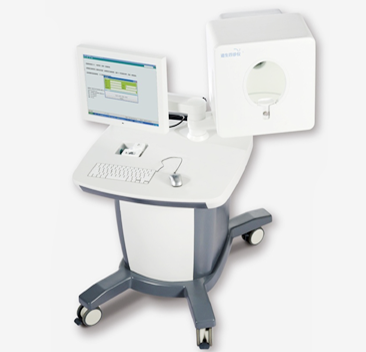
\includegraphics[height=6cm]{images/mzy.png}
    }
    \subfigure[云中医智能镜]{
        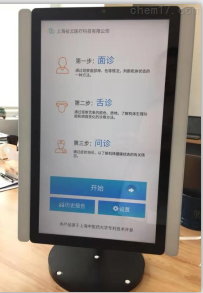
\includegraphics[height=6cm]{images/yzy.png}
    }
    \caption{读脸技术在医疗健康领域的应用}
    \label{fig:med}
\end{figure}
在医疗领域,读脸技术的应用主要还是供医护人员使用的系统。如在病人失去意识或者无法交流的情况下,利用读脸技术快速获取病人医疗信息的识别系统\cite{nwosu2016mobile},该系统基于人脸模板管理技和人脸匹配技术快速识别病人确定病人是否在数据库中,同时能够检索相关的医疗信息。Hossain, M. Shamim等\cite{Hossain2015Cloud}开发了一个利用语音和读脸技术,远程监控病人在家中健康状况的监控系统,不过该系统主要识别的是用户是否处于疼痛、紧张或者其他严重的状况等情况。面部特征进行健康监测的有面诊仪、云中医\cite{Zhang2018Study}等。面诊仪如道生面诊仪\cite{邸丹2016手持式舌象仪的研制}是目前某些医院用来采集面部信息的设备,需要在中医医师的指导下,进行舌相面色诊断信息采集,供中医医师进行判断; 在研究方面也有用面诊仪对冠心病的中医疗效进行评价的研究。如图 \ref{fig:med}所示,云中医是一个定点投放在诊所或者公共社区区域,可供用户进行中医面诊的系统,能够让用户在完成面诊舌诊问诊之后,给出健康分数和养生建议。
云中医虽然功能比较齐全,但是其主要应用场景是社区和诊所等公共环境,其中包括云中医诊断机器人\footnote{http://www.sohu.com/a/135358060_205169},云中医智能镜\cite{李雪2016},云中医应用\cite{钱鹏基于云中医的健康监测方法及系统}等,缺乏日常健康环境下的用户调研和交互研究。

\subsection{图像处理}
读脸技术还被用于面部图片处理。如为了促进购物,著名化妆品零售商Sephora开发了一个模拟化妆的系统,让用户可以在线查看各种化妆品的使用效果\cite{Sephora}。在当前小视频以及直播大火的时代,各类美颜技术和滤镜也被广泛使用。

\subsection{日常场景}
\begin{figure}[h]
    \centering
    \subfigure[微笑冰箱]{
        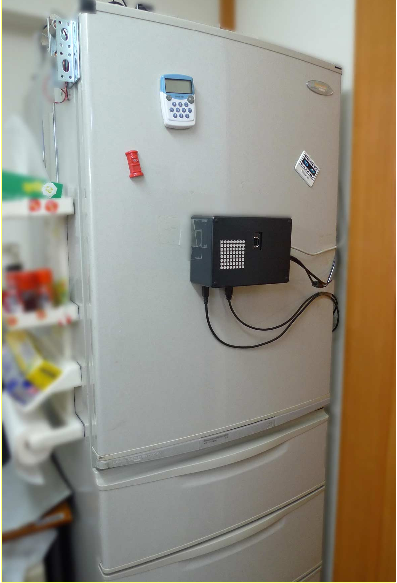
\includegraphics[width=4.5cm]{images/smile/6-Figure8-1.png}
    }
    \subfigure[SEMEOTICONS]{
        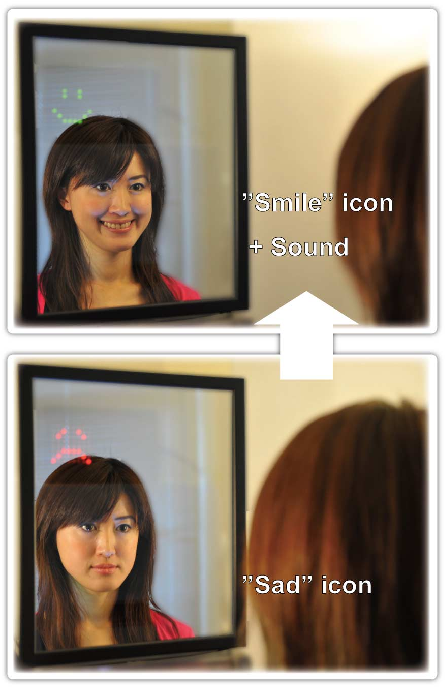
\includegraphics[width=4.5cm]{images/smile/2-Figure3-1.png}
    }
    \caption{读脸技术在日常场景下的应用}
    \label{fig:smile}
\end{figure}
相关研究也在探索如何将用户的日常行为和读脸技术结合起来。

如图 \ref{fig:smile} 所示,微笑冰箱\cite{Tsujita2011Smiling} 是一个通过冰箱上的设备能够监测到用户表情的冰箱,如果监测到用户打开冰箱是的面部是笑容则会自动解锁冰箱,该研究希望借此能够鼓励用户在日常生活中多微笑。 

\begin{figure}[h]
    \centering
    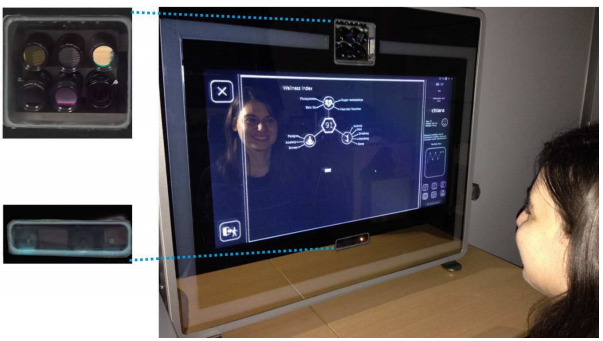
\includegraphics[width=12cm]{images/mirror.png}
    \caption{SEMEOTICONS}
    \label{fig:seme}
\end{figure}
如图 \ref{fig:seme} 所示,Yasmina Andreu-Cabedo等  \cite{andreu2015mirror}则开发了SEMEOTICONS, 一款放在家庭室内环境的镜子,通过采集面部信息和体温,监测与心血管疾病相关的户疲劳,压力和焦虑等特征, 让用户能够监测自己的健康情况,并根据量身定制的健康指南来改善用户的生活方式。
 该研究将面部信息和健康管理结合起来,并且将应用场景拓展到了日常环境。
 他们后续还进行了依次用户调研,调研结果表明\cite{coppini2017user} 他们的原型系统的设计被大多数用户所接受: 虽然测试过程非常耗时,大多数参与研究中的志愿者仍然很愿意完成并按计划进行实验,部分志愿者考虑了系统给出的健康指南,甚至因此改变了自己的生活方式。
总的来说,该系统通过将诊断和日常的照镜子的行为结合起来,可以很方便与用户的日常生活融合起来,但固定在房间的某个位置使用的方式不够便携,同时该系统需要一系列的传感器设备,也增加了硬件的成本,部署起来也相对麻烦,而且只能在室内使用。

\section{日常健康场景的交互研究}

从上一节我们可以知道,读脸技术在各个领域都有广泛的应用和研究,但是这些应用和研究却很少关注日常健康场景。而在人机交互领域,国内外有大量的关于如何设计日常场景下健康相关的交互研究。从研究目的来看,日常健康技术的研究重心偏向于关注患者的日常生活体验,加强患者与医护人员的协作,提高用户的疾病认知等方面\cite{nunes2015self-care}。
从研究的出发点来看,主要可以分为慢性疾病管理和鼓励用户健康生活方式的研究两种\cite{nunes2015self-care},本小节将从这两个方面展开分别介绍。

\subsection{慢性疾病管理}
在慢性疾病管理方面,当前研究主要是关于各种类型的慢性疾病的长期管理和追踪技术,提高用户在患病状态下的生活品质。
如 Lena Mamykina \cite{mamykina2008mahi:}团队在安卓平台上研发了一款称为 MAHI 的应用,通过蓝牙和传统的血糖仪进行通信,
提供了血糖记录的功能,并且允许用户之间在平台上互相交流等,经过实验发现该系统提供的功能能够大大鼓励用户实现血糖管理目标如控制饮食。
Kiyoshi Yasuda等人 \cite{yasuda2009remote}则研究了如何设计与痴呆病人的远程通讯系统,帮助痴呆病人与家人进行沟通,提高痴呆病人在家保持情绪稳定的时间,改善痴呆病人的日常在家的生活质量。
Amid Ayobi 等\cite{ayobi2017quantifying} 通过对多发性硬化病人的日常监测应用的研究,发现日常健康技术可以帮助提高病人的日常控制意识,而不只是监测疾病相关的指标。
在精神健康方面,Jakob E. Bardram等 \cite{bardram2013designing}探索了如何设计监测双相情感障碍症的日常应用, 研究发现因为移动平台的便携性,患者可以随时携带智能手机,通过系统提醒和实时数据可视化可以提高患者的疾病意识。
同时该系统提供的评估功能相较于纸质表格评估的模式,使用体验大大得到了提高,更加利于用户长期坚持疾病评估。

总的来说,健康管理和患者的日常生活密切相关,慢性病患者需要调整自己的饮食和锻炼等来实现有效的健康管理\cite{nunes2018understanding}。慢性病管理技术能够帮助用户了解病情的变化,及时对自己的病情变化做出应对行为,更好地评估自己的日常健康行为和更快地适应当前的生活状态\cite{ayobi2017quantifying}。


\subsection{健康行为引导}
在鼓励用户健康生活方面,主要是对各类监测系统的研究。这类系统的功能主要是对用户的各种健康比较相关的指标,能够让用户得到关于自己健康情况的一个反馈,
让用户处于健康或者亚健康的情况下,指导用户更加健康地生活。这类监测相关的技术,从监测的指标来看,可以大致分为两类:

(1) 日常行为的监控:通过监控用户的日常饮食、运动情况等日常行为,培养用户更好的饮食习惯、锻炼习惯\cite{purpura2011fit4life} \cite{Inagawa2013A} \cite{bravata2007using} \cite{cordeiro2015barriers} \cite{lin2006fish} \cite{miller2014stepstream}等。 例如Yuma Inagawa等人  \cite{Inagawa2013A} 开发了一个营养管理和检索系统,根据用户的喜好给出推荐的菜单,用户也可以给出对应的反馈,以此来培养用户健康的健康饮食的观念,进而达到引导用户的行为的效果。


(2) 健康指标的监控:健康指标主要包括血压、心率、睡眠\cite{kay2012lullaby} \cite{gronvall2013beyond} \cite{logan2007mobile} \cite{walters2010a}等。例如Stephen Purpura等人 \cite{purpura2011fit4life} 利用内有传感器的眼镜、耳机,臂环等可穿戴设备,通过记录用户的饮食、心率、咀嚼动作、体重、血压等健康指标,设计了一个鼓励用户减肥的系统 fit4life; Lullaby  \cite{kay2012lullaby} 是Matthew Kay等人利用光线、声音、温度、运动等传感器,用于研究干扰用户睡眠因素的系统,该系统通过记录和可视化用户的睡眠状态,能够帮助用户识别睡眠中断和环境因素之间的联系。 

% 总结上述的研究我们发现,当前关于日常健康交互技术的研究有很多,涉及各种慢性疾病管理以及各种健康评估和监测的方法,但是目前还缺乏关于日常环境下如何设计基于面部信息进行健康评估的研究。

不过目前这些健康追踪和监测技术,主要的实现方式还是通过量化采集用户的健康指标相关的数据。那么如何利用其他的健康相关数据,如面部信息,来支持用户的日常健康,在人机交互领域还没有得到深入研究。

% \section{健康诊断信息化技术}

% 目前的健康诊断相关技术,大多数还是应用在医疗环境下。

% 在信息化系统方面,相关的技术有电子病历管理系统\cite{高春芳2013电子病历系统应用现状及前景展望}, 电子影像管理系统\cite{张安平2018医院信息管理系统的电子病历和医学影像系统分析}, 医护信息管理系统\cite{虞正红2018医护合作静脉血栓栓塞管理信息化平台的设计与应用}等。
% 这些系统的主要目的是为了提高诊所内医生的工作效率,对相关的信息进行有效的管理。同时,这类管理系统因为是为医护从业人员设计,使用者需要丰富的专业知识和操作培训才能使用。

% 在医用器械研究方面,面诊仪如道生面诊仪\cite{邸丹2016手持式舌象仪的研制}是目前某些医院用来采集面部信息的设备,需要在中医医师的指导下,进行舌相面色诊断信息采集的设备,供中医医师进行判断;
%  同样,舌诊仪\cite{李丹溪2017舌诊仪的发展及其在舌诊客观化研究中的应用现状} 和脉诊仪 \cite{牛婷婷2017脉诊仪}虽然在电脑端会提供一些自动化分析的功能,但主要还是设计为辅助医师进行诊断或者数据采集的工具。
 
%  也有部分将诊断技术应用到日常环境下使用的工作。金姆脉诊仪\footnote{http://www.jinmuhealth.com/}是一个方便随身携带的脉诊设备,由信号采集器、移动端应用和服务端组成,信号采集器通过内部的光传感器记录用户的脉搏和脉象信号,移动端应用和信号采集器通过蓝牙连接,将数据发送给服务端,并展示来自服务端的结果。
%  用户将手指放入信号采集器中,系统通过脉象分析,就可以在移动端应用上看到自己的健康状况和对应的调理和治疗建议。
%  常见的智能穿戴设备,如小米公司开发的智能手环\footnote{http://www.mi.com/shouhuan4},除了手环本身带有手表的功能外,还支持了运动管理和健康管理,可以通过监测用户的心率脉搏和血压,给出用户的睡眠质量,甚至可以监测心脏健康等功能。
% 除了基于脉搏心率特征,还有基于面部特征进行健康监测的云中医\cite{Zhang2018Study}。云中医是一个定点投放在诊所或者公共社区区域,可供用户进行中医面诊的系统,能够让用户在完成面诊舌诊问诊之后,给出健康分数和养生建议。
%  云中医虽然功能比较齐全,但是其主要工作是算法和系统实现层面(其中包括云中医诊断机器人\footnote{http://www.sohu.com/a/135358060_205169},云中医智能镜\cite{李雪2016},云中医应用\cite{钱鹏基于云中医的健康监测方法及系统}等),缺乏深度的用户调研和交互研究。

% 以上提到的健康诊断技术,主要的实际应用场景还是局限在医疗诊所环境下,特别是面诊技术,没有考虑到普通用户的日常使用。在日常使用这种场景下,面诊技术有哪些独特的社会文化特点,用户会遇到哪些问题,相关的设计应该遵循哪些设计原则,还处于待研究的阶段。



\section{本章小结}
本章主要介绍了日常健康交互技术和读脸技术的相关工作。第一部分介绍了人机交互领域在日常健康方面的研究,从传统的慢性疾病管理到支持用户更健康生活方式的研究,同时指出当前的日常健康的研究,还未探索面部信息作为健康指标的技术。第二部分介绍了读脸技术的日常应用。随着技术的发展,读脸技术的应用非常广泛,从安防和访问控制,到情绪识别,也广泛用于医疗领域识别病人信息,远程监测患者, 甚至用于检测健康状态。但是医疗领域的读脸技术,大多是为专业医护人员设计的。关于日常健康场景下的面诊技术如何设计还需要进一步的探索。